%% IEEE TGRS submission -- Inductive GNN Transfer Learning for cross-city PM2.5
%% Compile: pdflatex main -> pdflatex main  (bibliography is embedded; no BibTeX needed)
%% Figures live in ../paper_figs/*.pdf
\documentclass[journal]{IEEEtran}

\usepackage{amsmath,amsfonts,amssymb}
\usepackage{algorithmic}
\usepackage{algorithm}
\usepackage{array}
\usepackage{booktabs}
\usepackage{multirow}
\usepackage{makecell}
\usepackage{graphicx}
\usepackage{textcomp}
\usepackage{xcolor}
\usepackage{url}
\usepackage{xspace}
\usepackage[caption=false,font=normalsize,labelfont=sf,textfont=sf]{subfig}
\usepackage[hidelinks]{hyperref}
\hyphenation{op-tical net-works semi-conduc-tor spatio-temporal}

\graphicspath{{../paper_figs/}}

% --- convenience macros ---------------------------------------------------
\newcommand{\pmf}{PM\textsubscript{2.5}\xspace}
\newcommand{\ugm}{\,$\mu$g\,m\textsuperscript{$-3$}\xspace}
\newcommand{\V}{\ensuremath{|V|}\xspace}
\newcommand{\Rtwo}{\ensuremath{R^{2}}\xspace}

\begin{document}

\title{Inductive Graph Neural Networks with Adversarial Domain Adaptation for Cross-City \pmf Forecasting under Heterogeneous Monitoring Topologies}

\author{Bishwadip~Maitra,~Subhojit~Mondal,~and~Mainak~Thakur%
\thanks{Bishwadip Maitra and Mainak Thakur are with the Department of Computer Science and Engineering, Indian Institute of Information Technology Sri City, Andhra Pradesh 517646, India (e-mail: bishwadip.maitra@iiits.in; mainak.thakur@iiits.in).}%
\thanks{Subhojit Mondal is with the Indian Institute of Technology Madras, Chennai 600036, India (e-mail: subhojit.mondal@smail.iitm.ac.in).}%
\thanks{\emph{Dummy e-mail addresses are placeholders to be finalized at submission.}}%
\thanks{Ground monitoring data were obtained from the Central Pollution Control Board (CPCB) Continuous Ambient Air Quality Monitoring network. Processed data and CPU-only code are released for reproducibility.}}

\markboth{IEEE Transactions on Geoscience and Remote Sensing (preprint)}%
{Maitra \MakeLowercase{\textit{et al.}}: Inductive GNN Transfer Learning for Cross-City \pmf Forecasting}

\maketitle

\begin{abstract}
Operational forecasting of fine particulate matter (\pmf) in many Indian cities is constrained by sparse and highly uneven ground-monitoring infrastructure: Delhi operates 40 Central Pollution Control Board (CPCB) stations, Kolkata 10, and Guwahati only 4. Transfer learning is a natural remedy for such data scarcity. We first establish, with a station-independent recurrent transfer model, that pre-training on a data-rich source city and fine-tuning on a small slice of a data-scarce target recovers most of the attainable accuracy from as little as 15\% of the target data --- evidence that transfer learning is a decisive lever for under-monitored cities. However, the station-independent recipe cannot exploit the spatial coupling between monitors, and its weights have no canonical reuse across cities with different station counts. We close both gaps with an inductive spatio-temporal graph neural network whose parameter count is independent of the number of stations, transferred across cities by two complementary strategies: supervised pre-train-and-fine-tune, and a novel Graph-DANN that adversarially aligns a size-invariant graph embedding. The single encoder trained on Delhi's 40-station graph operates verbatim on Guwahati's 4-station graph with no change of parameter shape. Across a grid of six ordered city pairs and four target-data fractions, every transfer cell is verified against both a zero-shot and a from-scratch baseline, passing in 24 of 24 cells for pre-train-and-fine-tune and 23 of 24 for Graph-DANN. The study is accompanied by a complete data-leakage and overfitting audit and runs end-to-end on commodity CPU hardware.
\end{abstract}

\begin{IEEEkeywords}
Air quality, particulate matter, spatio-temporal graph neural networks, transfer learning, domain adaptation, environmental monitoring networks, inductive learning.
\end{IEEEkeywords}

% =========================================================================
\section{Introduction}
% =========================================================================
\IEEEPARstart{F}{ine} particulate matter with aerodynamic diameter below 2.5\,$\mu$m (\pmf) is the leading environmental health risk worldwide \cite{hei2024}. India bears an acute share of this burden: in 2023 it ranked among the most polluted countries, and the National Capital Region of Delhi recorded an annual mean of roughly 100\ugm{}, about twenty times the World Health Organization guideline \cite{iqair2024,who2021}. Short-horizon (1--6\,h) \pmf forecasts are operationally critical: they trigger graded-response actions, inform school-closure and exposure advisories, and underpin public-health planning.

\textbf{The data-scarcity bottleneck.} The only public, real-time \pmf feed for most Indian cities is the CPCB Continuous Ambient Air Quality Monitoring (CAAQM) network, whose coverage is extremely unequal. Delhi has 40 stations in a single basin; Kolkata has 10 across a coastal--delta region; Guwahati, in the northeast, has only 4 in the Brahmaputra valley (Fig.~\ref{fig:study}). Most secondary cities have one station or none. A ``train one deep model per city'' recipe is therefore feasible only for a handful of Tier-1 cities, leaving the majority of the country without data-driven forecasting.

\textbf{Act~I --- transfer learning is a game-changer.} The natural remedy is transfer learning (TL): pre-train a forecaster on a data-rich source city and adapt it to a data-scarce target with a small fine-tune set. Our first contribution is to make this case concretely. Using a \emph{station-independent} long short-term memory (LSTM) forecaster shared across all monitors, we show that source pre-training plus fine-tuning on as little as 15\% of the target's training windows recovers \Rtwo within a few hundredths of the fully-supervised ceiling (Section~\ref{sec:results}). For a city with four monitors and a single year of data, this is the difference between a usable forecaster and none.

\textbf{Act~II --- but the station-independent form is architecturally capped.} The LSTM-TL model treats each monitor as an isolated univariate series and concatenates the predictions. Two consequences limit it. (i) \emph{Spatial coupling is ignored}: \pmf transports along wind corridors and forms regional plumes whose spatial structure carries genuine predictive signal \cite{wang2020pm25gnn}. (ii) \emph{The trained weights have no reusable spatial operator}: a ``model'' is a bundle of per-station forecasters, so the cross-station structure that differs between a 40-station and a 4-station city is never represented.

\textbf{Act~III --- inductive graph transfer closes the gap.} We therefore introduce a graph-TL framework that keeps what LSTM-TL achieves and additionally (i) learns a spatial operator over the monitoring graph and (ii) makes that operator transferable across cities of different size. The key is an \emph{inductive} spatio-temporal graph neural network (ST-GNN): no learnable parameter has a shape that depends on the number of nodes \V, so the same encoder transfers verbatim from a 40-station city to a 4-station one. The formal basis for cross-size transfer of such operators is the graphon-transferability result of Ruiz \emph{et al.}~\cite{ruiz2020graphon} and the spectral analysis of Levie \emph{et al.}~\cite{levie2021transfer}. We transfer the encoder by two strategies: supervised pre-train-and-fine-tune (PT-FT), and a novel \emph{Graph-DANN} that adversarially aligns a size-invariant graph embedding so that cities with \V differing by an order of magnitude become statistically indistinguishable before the small target gradient specializes.

\textbf{Contributions.}
\begin{itemize}
\item \textbf{C1.} A GNN-TL framework that, to our knowledge, is the first to transfer \pmf forecasters across cities whose monitoring-station counts differ by an order of magnitude (40\,$\leftrightarrow$\,10\,$\leftrightarrow$\,4). The inductive encoder ($\approx$25k parameters, no \V-shaped weights) operates on all three graphs without modification.
\item \textbf{C2.} \emph{Graph-DANN}, an adversarial domain-adaptation variant adapted to heterogeneous topologies through a size-invariant mean+max graph readout that lets a single discriminator compare cities of very different size.
\item \textbf{C3.} A strict three-way verification protocol: every reported transfer cell is compared against both a zero-shot baseline and a from-scratch baseline trained on the same target sub-sample, closing a falsifiability loophole common in cross-city TL.
\item \textbf{C4.} A complete data-leakage and overfitting audit, and CPU-only reproducible code; the full verification grid for each stage completes in $\approx$2.5\,h on 8 vCPU without a GPU.
\end{itemize}

The remainder is organized as follows. Section~\ref{sec:related} reviews related work; Section~\ref{sec:data} details the study area, instruments, and data; Section~\ref{sec:method} the forecasters and transfer strategies; Section~\ref{sec:setup} the experimental protocol; Section~\ref{sec:results} the results; Sections~\ref{sec:discussion}--\ref{sec:conclusion} discuss, bound, and conclude.

% =========================================================================
\section{Related Work}\label{sec:related}
% =========================================================================
\textbf{Graph neural networks for air quality.} PM2.5-GNN~\cite{wang2020pm25gnn} introduced wind-aware directed edges for nationwide Chinese \pmf forecasting; GAGNN~\cite{chen2021gagnn} added group-aware aggregation, HighAir~\cite{shao2021highair} a city--region hierarchy, and AirFormer~\cite{liang2023airformer} a stochastic transformer. None transfers across cities of substantially different station count; all are trained per region.

\textbf{Cross-city spatio-temporal transfer.} RegionTrans~\cite{wang2019regiontrans} introduced cross-city deep TL for traffic; MetaST~\cite{yao2019metast} and ST-GFSL~\cite{lu2022stgfsl} used meta-learning; CrossTReS~\cite{jin2022crosstres} re-weighted source regions; TransGTR~\cite{jin2023transgtr} learned cross-city graph structure. DASTNet~\cite{tang2022dastnet} is the closest precedent for adversarial cross-city transfer, but targets relatively homogeneous road networks. None treats order-of-magnitude \V-heterogeneity as a first-class concern.

\textbf{Inductive GNNs and domain-adversarial training.} GraphSAGE~\cite{hamilton2017graphsage} and GAT~\cite{velickovic2018gat} established the inductive paradigm; GIN~\cite{xu2019gin} grounds mean/max graph readouts. DANN~\cite{ganin2016dann} is the gradient-reversal paradigm we build on; ADDA~\cite{tzeng2017adda} contributes the source warm-start, and de~Mathelin \emph{et al.}~\cite{demathelin2020adversarial} explain why adversarial branches in \emph{regression} need loss reweighting. Within environmental time series, Yadav \emph{et al.}~\cite{yadav2024} use cross-year deep TL with attention on Delhi \pmf, the closest single-city precedent for our climatology-residual treatment; Sangiorgio and Guariso~\cite{sangiorgio2024} report TL gains for Alpine ozone. Table~\ref{tab:position} positions our work: to our knowledge no prior method simultaneously offers cross-city transfer under \V-heterogeneity, graph-level adversarial alignment, and a falsifiable verification protocol.

\begin{table}[!t]
\caption{Positioning Against the Closest Precedents}
\label{tab:position}
\centering
\footnotesize
\setlength{\tabcolsep}{4pt}
\begin{tabular}{lccccc}
\toprule
Method & \makecell{Cross-\\city} & \makecell{Het.\\\V} & \makecell{Graph\\adv.\,DA} & \makecell{3-way\\verif.} & Domain \\
\midrule
PM2.5-GNN \cite{wang2020pm25gnn}   & No  & ---      & No  & No  & \pmf \\
DASTNet \cite{tang2022dastnet}     & Yes & No       & Yes & No  & Traffic \\
ST-GFSL \cite{lu2022stgfsl}        & Yes & Partial  & No  & No  & Traffic \\
TransGTR \cite{jin2023transgtr}    & Yes & Partial  & No  & No  & Traffic \\
\textbf{This work}                 & \textbf{Yes} & \textbf{Yes (4--40)} & \textbf{Yes} & \textbf{Yes} & \textbf{\pmf} \\
\bottomrule
\end{tabular}
\end{table}

% =========================================================================
\section{Study Area, Instruments, and Data}\label{sec:data}
% =========================================================================

\begin{figure*}[!t]
\centering
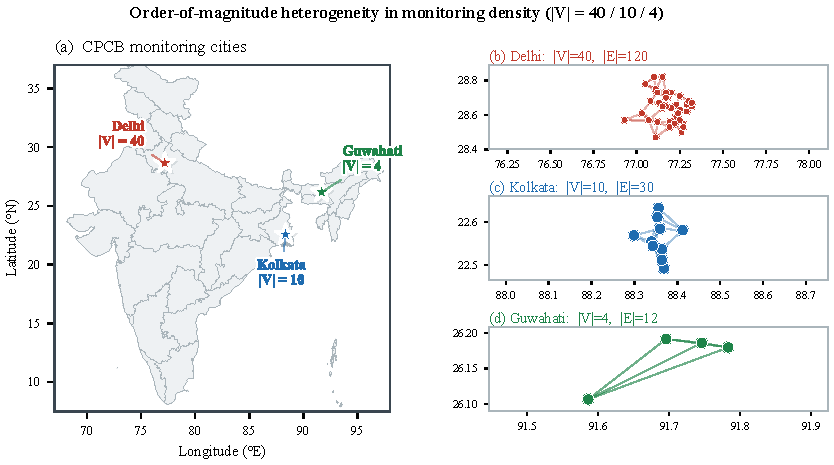
\includegraphics[width=\textwidth]{fig1_study_area.pdf}
\caption{Study area and monitoring-network heterogeneity. (a) The three CPCB cities on the Indian landmass; each marker reports the station count \V and the mean \pmf concentration. (b)--(d) Per-city $k$-nearest-neighbour station graphs ($k=3$) built from real station coordinates; \V ranges over $\{40,10,4\}$ at constant average degree. The same inductive encoder runs forward on all three.}
\label{fig:study}
\end{figure*}

\subsection{Study Area}
We study three Indian cities spanning distinct airshed regimes. \emph{Delhi} lies in the Indo-Gangetic Plain and experiences severe winter inversions (mean \pmf $\approx$\,101\ugm). \emph{Kolkata} is a humid coastal--delta city (mean $\approx$\,49\ugm). \emph{Guwahati} sits in the Brahmaputra valley with a pre-monsoon dust season and monsoon washout (mean $\approx$\,58\ugm). The geographic context and per-city monitoring graphs are shown in Fig.~\ref{fig:study}.

\subsection{Instruments and Data Acquisition}\label{sec:instruments}
All measurements come from the CPCB CAAQM network, India's reference real-time air-quality monitoring system. Each CAAQM station is a co-located instrument suite reporting at high frequency, which we aggregate to a uniform 3-hour cadence. The measured variables and their standard CAAQM instrumentation are:
\begin{itemize}
\item \textbf{\pmf} (\ugm), the forecast target, measured by continuous beta-attenuation monitors (BAM-class analysers) operating on the absorption of beta radiation by particulate mass collected on a filter tape, the CPCB reference-equivalent method for continuous \pmf;
\item \textbf{Air temperature} (AT, \textdegree C) and \textbf{relative humidity} (RH, \%) from a co-located thermo-hygrometer;
\item \textbf{Wind speed} (WS, m\,s\textsuperscript{$-1$}) and \textbf{wind direction} (WD, degrees) from a cup/vane or sonic anemometer.
\end{itemize}
Data were retrieved from the CPCB portal for Delhi over Jan.~2021--Dec.~2022 and for Kolkata and Guwahati over the 2023 monitoring year, giving $\approx$5840 three-hourly records per Delhi station and $\approx$2920 per Kolkata/Guwahati station. Station counts after quality screening are 40 (Delhi), 10 (Kolkata), and 4 (Guwahati); coordinates are in the WGS-84 datum. Table~\ref{tab:dataset} summarizes the dataset.

\begin{table}[!t]
\caption{Dataset and Monitoring-Graph Summary}
\label{tab:dataset}
\centering
\footnotesize
\begin{tabular}{lccccc}
\toprule
City & \V & $|E|$ & Period & 3-h steps & Mean \pmf \\
\midrule
Delhi    & 40 & 120 & 2021--2022 & $\approx$5840 & 101.5 \\
Kolkata  & 10 & 30  & 2023       & $\approx$2920 & 49.0 \\
Guwahati & 4  & 12  & 2023       & $\approx$2920 & 57.9 \\
\bottomrule
\end{tabular}
\end{table}

\subsection{Preprocessing and Feature Engineering}\label{sec:preproc}
Raw CAAQM feeds contain gaps from instrument downtime and quality flags, addressed by a two-stage spatio-temporal scheme following the predecessor study \cite{btp2025}.

\emph{Spatial interpolation (IDW).} A missing reading at station $s_0$ and time $t$ is first estimated from the $M$ nearest valid stations by inverse-distance weighting,
\begin{equation}
\hat{y}(s_0,t)=\frac{\sum_{m=1}^{M} d(s_0,s_m)^{-p}\,y(s_m,t)}{\sum_{m=1}^{M} d(s_0,s_m)^{-p}},\qquad p=2,
\label{eq:idw}
\end{equation}
where $d(\cdot,\cdot)$ is the great-circle distance, so nearer monitors dominate the estimate.

\emph{Temporal smoothing (Kalman).} Each station series is then passed through a local-level Kalman filter with latent state $x_t$ and observation $z_t$,
\begin{equation}
x_t = x_{t-1}+\omega_t,\ \ \omega_t\!\sim\!\mathcal{N}(0,Q);\qquad z_t = x_t+\nu_t,\ \ \nu_t\!\sim\!\mathcal{N}(0,R),
\label{eq:kfmodel}
\end{equation}
propagated by the standard predict--update recursion
\begin{equation}
\begin{aligned}
&\hat{x}_{t|t-1}=\hat{x}_{t-1}, &&P_{t|t-1}=P_{t-1}+Q,\\
&K_t=\frac{P_{t|t-1}}{P_{t|t-1}+R}, && \hat{x}_t=\hat{x}_{t|t-1}+K_t\big(z_t-\hat{x}_{t|t-1}\big),
\end{aligned}
\label{eq:kf}
\end{equation}
with $P_t=(1-K_t)P_{t|t-1}$. The filter denoises the series and fills short gaps by emitting the one-step prediction $\hat{x}_{t|t-1}$ whenever $z_t$ is absent. A final causal forward-fill using train-period statistics closes any residual gap without anticausal leakage (Section~\ref{sec:setup}).

\emph{Feature engineering.} We then form $F=14$ features per (station, step): \pmf, AT, RH, WS, the Cartesian wind-direction pair $(\sin\phi,\cos\phi)$, the cyclic time encodings
\begin{equation}
\Big(\sin\tfrac{2\pi h}{24},\ \cos\tfrac{2\pi h}{24},\ \sin\tfrac{2\pi m}{12},\ \cos\tfrac{2\pi m}{12}\Big)
\label{eq:cyclic}
\end{equation}
for hour $h$ and month $m$, and four India-specific season indicators. All features are standardized with statistics fit on the training partition only.

\emph{Climatology-residual target.} Let $c_n(m,h)$ be the per-(month, hour) mean \pmf at station $n$, estimated on the training slice. Rather than predicting raw \pmf, the network regresses the standardized \emph{anomaly}
\begin{equation}
\tilde{y}_{n,t}=\frac{\big(y_{n,t}-c_n(m_t,h_t)\big)-\mu_{\mathrm{tr}}}{\sigma_{\mathrm{tr}}},
\label{eq:resid}
\end{equation}
and a prediction is mapped back by $\hat{y}_{n,t}=\sigma_{\mathrm{tr}}\,\hat{\tilde{y}}_{n,t}+\mu_{\mathrm{tr}}+c_n(m_t,h_t)$. Removing the strong diurnal/seasonal climatology before learning suppresses the dominant cross-city, cross-year mean shift, leaving the harder anomaly component for the model and, as we show in Section~\ref{sec:setup}, rendering the residual series approximately stationary.

\subsection{Graph Construction}\label{sec:graph}
City $c$ induces a directed graph $\mathcal{G}_c=(\mathcal{V}_c,\mathcal{E}_c,W_c)$ whose $|\mathcal{V}_c|=N_c$ nodes are the stations. An edge $(i\!\rightarrow\!j)\in\mathcal{E}_c$ exists iff station $i$ is among the $k=3$ nearest neighbours of $j$ by great-circle (haversine) distance $d_{ij}$, with Gaussian-decay weight
\begin{equation}
w_{ij}=\exp\!\left(-\,d_{ij}^{2}/(2\sigma^{2})\right),\qquad \sigma=5~\text{km},
\label{eq:edge}
\end{equation}
collected in the sparse weight matrix $W_c\in\mathbb{R}^{N_c\times N_c}$. This yields the per-city graphs of Fig.~\ref{fig:study} and Table~\ref{tab:dataset}, all at constant average degree $3.0$ (so $|\mathcal{E}_c|=kN_c$). Crucially, only the \emph{weights} are city-specific; the operator that consumes them (Section~\ref{sec:encoder}) is shared.

\subsection{Problem Formulation}\label{sec:problem}
Let a city have $N$ stations and $F$ features. Given a history of $H=8$ steps (24\,h), we predict \pmf one horizon step ahead (+3\,h) at every station:
\begin{equation}
f_{\theta}:\ \mathbb{R}^{H\times N\times F}\ \rightarrow\ \mathbb{R}^{N}.
\label{eq:map}
\end{equation}
The architecture of Section~\ref{sec:method} instantiates $f_\theta$ so that the parameter count of $\theta$ is \emph{independent of} $N$; the same trained $\theta$ thus operates on Delhi, Kolkata, and Guwahati without shape change.

% =========================================================================
\section{Methodology}\label{sec:method}
% =========================================================================

\begin{figure*}[!t]
\centering
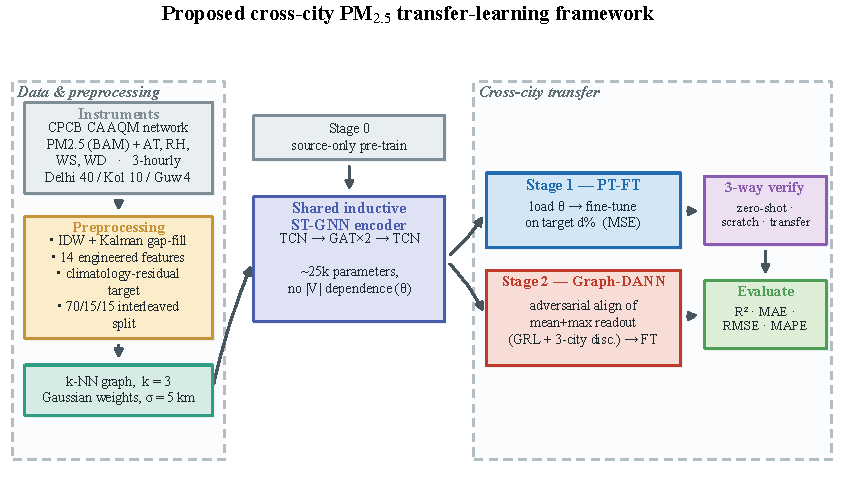
\includegraphics[width=\textwidth]{fig2_framework.pdf}
\caption{Proposed cross-city \pmf transfer-learning framework. CPCB instrument feeds are harmonized and converted to a climatology-residual target under an interleaved split; a per-city $k$-NN graph is built. A single inductive ST-GNN encoder is pre-trained on a source city (Stage~0) and transferred to a data-scarce target either by supervised fine-tuning (Stage~1, PT-FT) or by adversarial domain adaptation (Stage~2, Graph-DANN). Every cell passes three-way verification before evaluation on the target test partition.}
\label{fig:framework}
\end{figure*}

Fig.~\ref{fig:framework} gives the end-to-end framework. We study two forecasters --- a station-independent LSTM-TL model and the inductive ST-GNN --- and two graph-transfer strategies. Both forecasters realize \eqref{eq:map} with a parameter count independent of $N$.

\subsection{Inductive ST-GNN Encoder}\label{sec:encoder}
The encoder is a four-block stack \mbox{TCN\,$\rightarrow$\,GAT\,$\times$2\,$\rightarrow$\,TCN\,$\rightarrow$\,Linear} (Fig.~\ref{fig:encoder}), in the STGCN/Graph-WaveNet family \cite{yu2018stgcn,wu2019graphwavenet}, kept small ($\approx$25k parameters) for CPU compute. It interleaves a \emph{temporal} step that summarizes each station's recent hours and a \emph{spatial} step that refines each station's state from a learned weighted average of its neighbours.

\textbf{TemporalConv.} A 1-D causal convolution of kernel size $K=3$ applied per node along time,
\begin{equation}
\big(\mathrm{TConv}\,x\big)_{n,t,:}=\sum_{k=0}^{K-1}\Theta_k\,x_{n,\,t-\delta k,\,:}+b,
\label{eq:tconv}
\end{equation}
with kernels $\Theta_k\in\mathbb{R}^{d_{\text{in}}\times d_{\text{out}}}$, left-padded and causally trimmed so output step $t$ depends only on inputs at steps $\le t$. The two blocks use dilation $\delta\in\{1,2\}$ (TCN primitive of \cite{bai2018tcn}); the second has a receptive field of 7 of the 8 history steps.

\textbf{Edge-weighted GAT.} For each directed edge $i\!\rightarrow\!j$ the attention logit injects the external edge weight log-additively,
\begin{equation}
e_{ij}=\mathrm{LeakyReLU}\!\left(a_s^{\top}Wx_i + a_d^{\top}Wx_j\right)+\log w_{ij},
\label{eq:gat}
\end{equation}
which a per-destination softmax normalizes before aggregation,
\begin{equation}
\alpha_{ij}=\frac{\exp(e_{ij})}{\sum_{i'\in\mathcal{N}(j)}\exp(e_{i'j})},\qquad
h_j=\sum_{i\in\mathcal{N}(j)}\alpha_{ij}\,Wx_i.
\label{eq:agg}
\end{equation}

\textbf{Size-invariant readout (Stage~2).} A graph-level embedding is formed by concatenating mean and max pooling over the node axis of the last-step hidden state,
\begin{equation}
z=\big[\,\mathrm{mean}_{n}\,h_{T}[\,:,n,:]\ \big\Vert\ \mathrm{max}_{n}\,h_{T}[\,:,n,:]\,\big],
\label{eq:readout}
\end{equation}
the GIN-style readout \cite{xu2019gin} that lets a single discriminator compare cities of very different size.

\begin{figure}[!t]
\centering
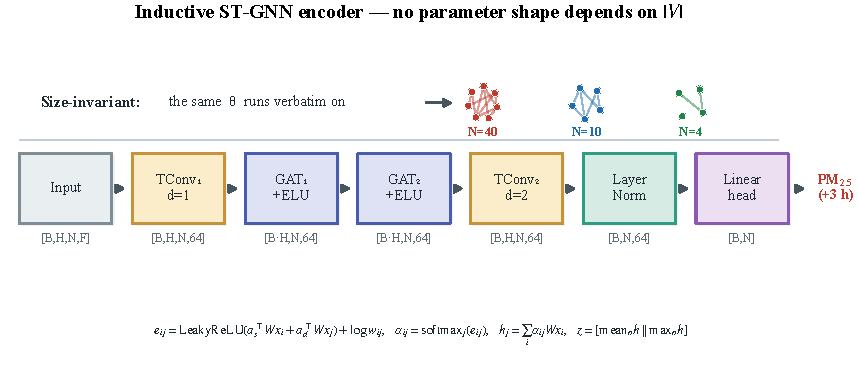
\includegraphics[width=\columnwidth]{fig3_encoder.pdf}
\caption{Inductive ST-GNN encoder. Every parameter's shape depends only on $(F, d_{\text{hidden}}, d_{\text{gat}})$, never on \V, so the same $\approx$25k-parameter $\theta$ runs verbatim on $N=40,10,4$ (Table~\ref{tab:params}).}
\label{fig:encoder}
\end{figure}

\textbf{Composed forward pass.} Writing $X\in\mathbb{R}^{B\times H\times N\times F}$ for a mini-batch of input windows, the encoder composes the temporal and spatial primitives as
\begin{equation}
\begin{aligned}
U &= \mathrm{TConv}_2\!\big(\mathrm{GAT}_2\circ\mathrm{GAT}_1\circ\mathrm{TConv}_1(X)\big),\\
h &= \mathrm{LayerNorm}(U)_{:,H,:,:},\qquad \hat{\tilde{y}} = h\,W_o+b_o,
\end{aligned}
\label{eq:forward}
\end{equation}
where the GAT layers \eqref{eq:gat}--\eqref{eq:agg} act on each of the $B{\cdot}H$ per-timestep graphs (the time axis folded into the batch), the temporal convolutions \eqref{eq:tconv} mix only along time per node, $h\in\mathbb{R}^{B\times N\times d_h}$ is the last-step hidden state, and $W_o\in\mathbb{R}^{d_h\times 1}$ is the shared output head.

\textbf{Why it is inductive.} Table~\ref{tab:params} enumerates the parameter shapes; none contains an $N$-dependent term, which we state as follows.

\smallskip
\noindent\textbf{Proposition~1 (Size-invariance).} \emph{Every learnable tensor in \eqref{eq:gat}--\eqref{eq:forward} has a shape determined only by $(F,d_h,d_g,K)$ and independent of the node count $N$; consequently $f_\theta$ is well-defined on a graph of any size and a single $\theta$ applies to $\mathcal{G}_{\mathrm{Delhi}}$, $\mathcal{G}_{\mathrm{Kolkata}}$, and $\mathcal{G}_{\mathrm{Guwahati}}$.}

\smallskip
\noindent\textit{Proof sketch.} The node count $N$ enters \eqref{eq:tconv}--\eqref{eq:forward} only as a batched axis. The temporal kernels $\Theta_k$ act identically per node; the GAT projections $W,a_s,a_d$ act per node and per edge; the readout \eqref{eq:readout} and the output head $W_o$ aggregate or map along the feature axis. No parameter indexes a node identity or has $N$ in its shape, so the counts of Table~\ref{tab:params} carry no $N$ term. The same checkpoint therefore loads onto Delhi's 40-station and Guwahati's 4-station graphs unchanged --- the mechanical precondition for Stages~1 and 2. $\hfill\blacksquare$

\begin{table}[!t]
\caption{Parameter Shapes ($d_{\text{hidden}}=d_{\text{gat}}=64$)}
\label{tab:params}
\centering
\footnotesize
\begin{tabular}{lccr}
\toprule
Component & Shape & Depends on \V? & Count \\
\midrule
TemporalConv$_1$ & $(F,64,3)$ & No & $\sim$2.7k \\
GAT$_1$ ($W,a_s,a_d$) & $(64,64),(64),(64)$ & No & $\sim$4.3k \\
GAT$_2$ ($W,a_s,a_d$) & $(64,64),(64),(64)$ & No & $\sim$4.3k \\
TemporalConv$_2$ & $(64,64,3)$ & No & $\sim$12.4k \\
LayerNorm + head & $(64),(64),(64,1)$ & No & $\sim$0.2k \\
\midrule
\textbf{Total} & --- & \textbf{No} & \textbf{$\sim$25k} \\
\bottomrule
\end{tabular}
\end{table}

\subsection{Station-Independent LSTM-TL Baseline}\label{sec:lstm}
The Act-I forecaster treats every monitor as an independent univariate problem. A single 2-layer LSTM (hidden 64, dropout 0.2), \emph{shared across all stations}, reads a station's 24-h history and predicts its next value. Per step, the cell computes
\begin{equation}
\begin{aligned}
i_t,f_t,o_t &= \sigma\!\left(W[h_{t-1},x_t]+b\right),\quad
g_t = \tanh\!\left(W_g[h_{t-1},x_t]+b_g\right),\\
c_t &= f_t\odot c_{t-1}+i_t\odot g_t,\qquad h_t = o_t\odot\tanh(c_t),
\end{aligned}
\label{eq:lstm}
\end{equation}
and a two-layer head maps $h_H$ to the +3\,h prediction. Because the same weights ($\approx$50k, independent of $N$) are applied to each station and nothing refers to station identity, the network transfers to a new city by simply running on its stations --- clean, but unable to represent any coupling \emph{between} stations.

\subsection{Cross-City Transfer}\label{sec:transfer}
\textbf{Stage~0 (pre-training).} For each city, the encoder is trained on the full training partition with mean-squared error in z-scored climatology-residual space, Adam, weight decay $10^{-5}$, gradient clipping at norm 1, \texttt{ReduceLROnPlateau} on validation \Rtwo, and best-by-validation checkpointing.

\textbf{Stage~1 (PT-FT).} The source checkpoint is loaded into a target-instantiated encoder; the input TemporalConv is frozen for the first 20\% of fine-tune epochs (frozen-low-layers convention \cite{yosinski2014}) then unfrozen. Fine-tuning uses $d\%$ of the target training windows, $d\in\{15,30,45,60\}$. For LSTM-TL the same recipe runs without the freeze step.

\textbf{Stage~2 (Graph-DANN).} Stage~2 wraps the encoder with a gradient-reversal layer (GRL) and a 3-class city discriminator $D_{\theta_d}$ over the size-invariant embedding \eqref{eq:readout} (Fig.~\ref{fig:dann}). The GRL $\mathcal{R}_\lambda$ is the identity in the forward pass and negates-and-scales the gradient in the backward pass,
\begin{equation}
\mathcal{R}_\lambda(z)=z,\qquad \frac{\partial \mathcal{R}_\lambda}{\partial z}=-\lambda\,I,
\label{eq:grl}
\end{equation}
so a single descent step trains $D_{\theta_d}$ to name the city while training the encoder to \emph{erase} city identity from $z$. With encoder, forecast-head, and discriminator parameters $(\theta_e,\theta_y,\theta_d)$, the joint phase seeks the saddle point
\begin{equation}
\min_{\theta_e,\theta_y}\ \max_{\theta_d}\ \ \mathcal{L}_{\mathrm{MSE}}(\theta_e,\theta_y)\ -\ \alpha_d\,\mathcal{L}_{\mathrm{CE}}(\theta_e,\theta_d),
\label{eq:minmax}
\end{equation}
realized per mini-batch by the composite loss
\begin{equation}
\mathcal{L}=\mathrm{MSE}(\hat{y},y)+\alpha_d\big(\mathrm{CE}_{\text{src}}+\mathrm{CE}_{\text{tgt}}+\mathrm{CE}_{\text{3rd}}\big),
\label{eq:dann}
\end{equation}
where the GRL implements \eqref{eq:minmax} by passing $-\lambda$ times the discriminator gradient into the encoder. Three mini-batches (source, target with labels withheld, third-city replay) are processed per step, each on its own graph. A logistic warm-up
\begin{equation}
\lambda(p)=\frac{2}{1+\exp(-\gamma p)}-1,\quad p=\tfrac{\text{step}}{\text{total}},\ \gamma=10,
\label{eq:lambda}
\end{equation}
lets the forecaster stabilize before the adversary saturates. After the joint phase the GRL is disabled ($\lambda=0$) and the model is fine-tuned on $d\%$ of the target labels with the Stage-1 recipe. Stabilization choices --- source warm-start \cite{tzeng2017adda}, discriminator reweighting $\alpha_d=0.1$ \cite{demathelin2020adversarial}, and pre-GRL normalization --- are detailed in the supplement.

\begin{figure}[!t]
\centering

\includegraphics[width=\columnwidth]{fig4_graph_dann.pdf}
\caption{Graph-DANN. A round-robin three-city minibatch feeds the shared encoder; its size-invariant readout $z$ branches into a forecast head (MSE) and, through a gradient-reversal layer, a 3-way city discriminator (CE). The encoder is trained to \emph{fool} the discriminator, producing a city-invariant embedding. Inset: the $\lambda(p)$ warm-up.}
\label{fig:dann}
\end{figure}

\subsection{Stage~3 --- Dual Transfer Learning}\label{sec:dual}
Graph-DANN aligns only the \emph{marginal} embedding distribution $P(z)$, and on our grid it merely ties PT-FT (Section~\ref{sec:results}). This is expected rather than anomalous: for \emph{regression} --- unlike classification --- aligning representation distributions alters feature scale and impedes adaptation \cite{chen2021rsd}, and adversarial regression alignment requires heavy down-weighting to avoid harm \cite{demathelin2020adversarial}. Following the marginal/conditional duality of \emph{dual transfer learning} \cite{long2012dtl}, we add a second, complementary alignment to the marginal adversary and study two instantiations.

\textbf{Dual-CDAN (conditional adversary).} In the spirit of conditional adversarial adaptation \cite{long2018cdan}, a second discriminator is conditioned on the forecast through the multilinear map
\begin{equation}
T = z \otimes g(\hat{y}),\qquad g(\hat{y})=\mathrm{MLP}\big([\,\mathrm{mean}_n\,\hat{y}\ \Vert\ \mathrm{std}_n\,\hat{y}\,]\big),
\label{eq:cdan}
\end{equation}
so the encoder is pressed to make the \emph{joint} $(z,\hat{y})$ distribution city-invariant rather than $z$ alone.

\textbf{Dual-RSD (subspace alignment).} We instead add the scale-free Representation Subspace Distance \cite{chen2021rsd} between the source and target embedding batches $Z_s,Z_t$. Orthonormal bases $Q_s,Q_t$ of the two embedding subspaces are obtained by QR; the cosines of the principal angles $\Theta$ are the singular values of $Q_s^{\top}Q_t$, and the distance is the Grassmann projection metric
\begin{equation}
\mathrm{RSD}(Z_s,Z_t)=\lVert\sin\Theta\rVert_1,\qquad \cos\Theta=\mathrm{svdvals}\!\left(Q_s^{\top}Q_t\right),
\label{eq:rsd}
\end{equation}
which aligns the \emph{geometry} of the representations without altering their scale --- the property \cite{chen2021rsd} identifies as essential for regression. The dual joint objective is
\begin{equation}
\mathcal{L}_{\text{dual}}=\mathrm{MSE}(\hat{y},y)+\alpha_m\,\mathcal{L}^{\text{marg}}_{\mathrm{CE}}+\beta\,\mathrm{RSD}(Z_s,Z_t),
\label{eq:dualobj}
\end{equation}
with the marginal term as in \eqref{eq:dann} and $\beta=0.05$. Both variants reuse the Stage-2 protocol (warm-start, $\lambda$ schedule, fine-tune); only the alignment term changes. Related conditional/joint-distribution methods include JAN \cite{long2017jan} and subdomain LMMD \cite{zhu2021dsan}.

\subsection{Three-Way Verification Protocol}\label{sec:verify}
A cell demonstrates \emph{real} transfer only if the transfer model beats \emph{both} a zero-shot baseline (source weights, no fine-tune) and a from-scratch baseline (random init, same target sub-sample). Algorithm~\ref{alg:verify} formalizes this; the scratch control closes a loophole in much cross-city TL, where reporting only the transfer score cannot separate ``the source helped'' from ``we simply trained on $d\%$ of the target.''

\begin{algorithm}[!t]
\caption{Three-way verification per $(s,t,d)$ cell}
\label{alg:verify}
\begin{algorithmic}[1]
\STATE \textbf{Input:} source checkpoint $\theta_s$, target city $t$, fraction $d$
\STATE $X,y \leftarrow$ target training windows for $t$
\STATE $\mathrm{keep}\leftarrow \mathrm{rng}(42).\mathrm{choice}(|X|,\lceil d|X|\rceil)$
\STATE $X_{ft},y_{ft}\leftarrow X[\mathrm{keep}],y[\mathrm{keep}]$
\STATE $R^2_{zs}\leftarrow \mathrm{eval}(\theta_s,\ t.\text{test})$ \hfill // zero-shot
\STATE $\theta_{tl}\leftarrow \mathrm{finetune}(\theta_s, X_{ft},y_{ft})$;\quad $R^2_{tl}\leftarrow \mathrm{eval}(\theta_{tl},\ t.\text{test})$
\STATE $\theta_{sc}\leftarrow \mathrm{train\_scratch}(X_{ft},y_{ft})$;\quad $R^2_{sc}\leftarrow \mathrm{eval}(\theta_{sc},\ t.\text{test})$
\STATE \textbf{return} $\mathrm{real}\leftarrow (R^2_{tl}>R^2_{zs})\wedge(R^2_{tl}>R^2_{sc})$
\end{algorithmic}
\end{algorithm}

We summarize a cell by the \emph{transfer gain} over the stronger baseline,
\begin{equation}
\Delta = R^2_{tl}-\max\!\big(R^2_{zs},\,R^2_{sc}\big),
\label{eq:gain}
\end{equation}
so a cell shows real transfer iff $\Delta>0$; we report the mean $\Delta$ over the grid alongside the pass count.

\subsection{Computational Complexity and Transferability}\label{sec:complexity}
\textbf{Time.} A forward pass costs $\mathcal{O}\!\big(BH\,(N d_h^2 + |\mathcal{E}|\,d_g)\big)$: the temporal convolutions \eqref{eq:tconv} are $\mathcal{O}(N d_h^2)$ per step and the sparse attention \eqref{eq:gat}--\eqref{eq:agg} is $\mathcal{O}(|\mathcal{E}|\,d_g)$, linear in the number of edges. Because the $k$-NN graph has $|\mathcal{E}|=kN$, the encoder scales \emph{linearly} in the station count: a 40-station city costs an order of magnitude more than a 4-station city, not the quadratic blow-up of a dense pairwise model. This is what keeps the full 24-cell grid within $\approx$2.5\,h on CPU.

\textbf{Parameters.} Summing Table~\ref{tab:params}, $|\theta|=\mathcal{O}(F d_h K + d_h d_g)$, with no $N$ term (Proposition~1) --- the precondition for loading one checkpoint onto graphs of different size.

\textbf{Transferability.} The empirical cross-$N$ behaviour is consistent with the graphon-transferability bound of Ruiz \emph{et al.}~\cite{ruiz2020graphon}: if two graphs are sampled from graphons $W_1,W_2$ close in cut norm, an inductive GNN $\Phi$ obeys
\begin{equation}
\big\lVert \Phi(\mathcal{G}_1)-\Phi(\mathcal{G}_2)\big\rVert \le \kappa_1\,\lVert W_1-W_2\rVert_{\square}+\kappa_2\!\left(N_1^{-1}+N_2^{-1}\right),
\label{eq:transfer}
\end{equation}
for Lipschitz constants $\kappa_1,\kappa_2$. The CPCB $k$-NN station graphs of the Indo-Gangetic and Brahmaputra airsheds plausibly satisfy the closeness premise, and the $24/24$ PT-FT pass rate validates the conclusion in the tested regime; we do not claim it holds for arbitrary graph pairs.

% =========================================================================
\section{Experimental Setup}\label{sec:setup}
% =========================================================================
\textbf{Splits.} We use a deterministic interleaved 70/15/15 split (every 7th step to validation, every 7th to test, disjoint), adopted because Kolkata and Guwahati have a single year of data, for which a chronological-tail test partition would be winter-only. Fine-tuning draws $d\%$ random sub-samples with a fixed seed; the same sub-sample is reused across the three trainings of a cell so verification is comparable per cell.

\textbf{Baselines.} The cross-method comparator is our station-independent LSTM-TL under the identical protocol (interleaved split, climatology residual, per-city recipe), so any protocol effect cancels at comparison time. Per-cell controls are zero-shot and scratch (Section~\ref{sec:verify}).

\textbf{Hyperparameters.} Table~\ref{tab:hyper} lists the per-stage configuration. Common to all runs: Adam, weight decay $10^{-5}$, gradient clip 1.0, dropout 0.15, hidden/GAT dim 64, single attention head, \texttt{ReduceLROnPlateau}$(0.5,3)$, seed 42.

\begin{table}[!t]
\caption{Hyperparameter Configuration}
\label{tab:hyper}
\centering
\footnotesize
\begin{tabular}{llcccc}
\toprule
Stage & City & Epochs & Batch & LR & Patience \\
\midrule
\multirow{3}{*}{Source GNN} & Delhi & 25 & 128 & $1\!\times\!10^{-3}$ & 6 \\
 & Kolkata & 40 & 64 & $1\!\times\!10^{-3}$ & 8 \\
 & Guwahati & 60 & 32 & $5\!\times\!10^{-4}$ & 10 \\
\midrule
\multirow{3}{*}{Fine-tune} & Delhi & 25 & 128 & $2\!\times\!10^{-4}$ & 6 \\
 & Kolkata & 30 & 64 & $2\!\times\!10^{-4}$ & 8 \\
 & Guwahati & 40 & 32 & $1\!\times\!10^{-4}$ & 10 \\
\midrule
Graph-DANN joint & --- & 25 & 32/city & $5\!\times\!10^{-4}$ & --- \\
\bottomrule
\end{tabular}
\end{table}

\textbf{Metrics and software.} Per-cell \Rtwo, MAE, RMSE, and MAPE are computed in raw \pmf space after inverse z-scoring and climatology add-back. The implementation is PyTorch with NumPy and scikit-learn only --- no PyTorch Geometric or compiled extensions --- so the full 24-cell grid for each stage completes in $\approx$2.5\,h on 8 vCPU, 16\,GB, no GPU.

\textbf{Leakage and overfitting audit.} Scalers and the per-(month, hour) climatology are fit on the training mask only; an in-loader imputation was patched to be strictly causal (verified bit-identical on the pre-imputed data). Window histories may overlap split boundaries but each supervision target is uniquely owned by one split, which is asymptotically valid for the (climatology-removed, approximately stationary) series \cite{bergmeir2018cv}. The validation$-$test \Rtwo gap averages $-0.005$ (test slightly above validation), indicating no overfitting. The full line-by-line audit is released as supplementary material.

% =========================================================================
\section{Results and Analysis}\label{sec:results}
% =========================================================================
All metrics are on the target city's held-out test partition in raw \pmf space. The grid per stage is six ordered (source, target) pairs $\times$ four target fractions.

\subsection{Source-Only Forecasters}
Both forecasters reach \Rtwo $\approx 0.82$--$0.86$ on all three cities, \emph{including the 4-station Guwahati graph} (Table~\ref{tab:source}), confirming the inductive encoder operates correctly at every \V. The LSTM is marginally ahead on single-city fit; the GNN's distinctive value is structural cross-\V transfer, shown next.

\begin{table}[!t]
\caption{Source-Only Test \Rtwo\,/\,MAE (\ugm) per City}
\label{tab:source}
\centering
\footnotesize
\begin{tabular}{lcc}
\toprule
City & LSTM & GAT-GNN \\
\midrule
Delhi    & \textbf{0.850}\,/\,23.7 & 0.834\,/\,24.2 \\
Kolkata  & \textbf{0.863}\,/\,\phantom{0}7.8 & 0.824\,/\,\phantom{0}9.2 \\
Guwahati & \textbf{0.832}\,/\,12.2 & 0.831\,/\,12.8 \\
\bottomrule
\end{tabular}
\end{table}

\subsection{Act~I: Transfer Learning Is a Game-Changer (LSTM-TL)}
Under the fixed protocol, LSTM-TL recovers strong target accuracy from very little target data: e.g., Delhi$\rightarrow$Kolkata reaches \Rtwo$=0.844$ at $d=15\%$ and $0.857$ at $d=60\%$, and Guwahati targets exceed $0.81$ from $d=15\%$. For a 4-station, single-year city, this turns an infeasible per-city model into a deployable forecaster. This establishes the central premise: \emph{TL is the decisive lever for data-scarce cities}. What it cannot do --- exploit spatial coupling or reuse a spatial operator across sizes --- motivates the graph model.

\subsection{Act~II/III: GNN-TL Stage~1 (PT-FT) and Verification}
Table~\ref{tab:cross} (columns S1) reports Stage-1 transfer at $d=30\%$; the best cell is Delhi$\rightarrow$Guwahati at $d=45\%$ (\Rtwo$=0.827$). Critically, \textbf{all 24 PT-FT cells pass three-way verification} (mean gain over scratch $+0.022$\,\Rtwo), visualized in Fig.~\ref{fig:verify}: in every cell the transfer panel exceeds both the zero-shot and scratch panels, and the data-efficiency curves show the transfer advantage is largest precisely where target data is scarcest.

\begin{figure*}[!t]
\centering
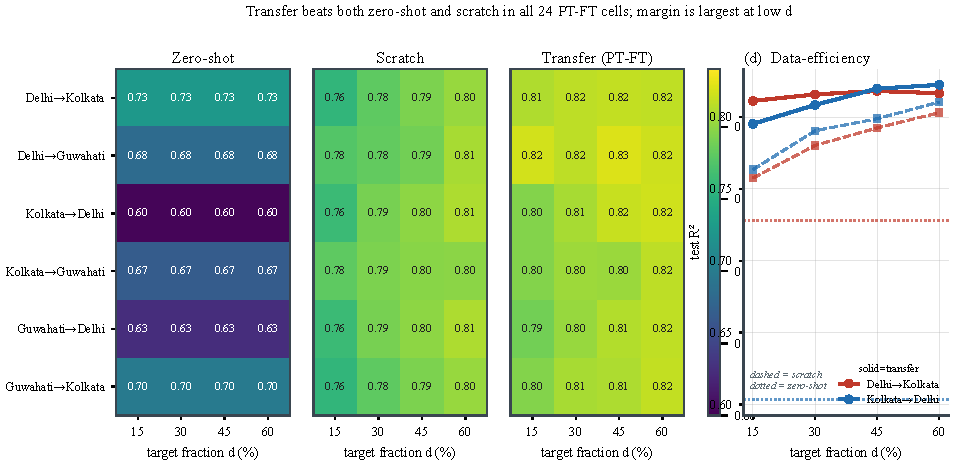
\includegraphics[width=\textwidth]{fig5_verification.pdf}
\caption{Three-way verification of Stage-1 PT-FT across the 24-cell grid (shared colour scale). In all 24 cells the transfer panel exceeds both the zero-shot and from-scratch panels. (d) Data-efficiency: transfer (solid) dominates scratch (dashed) and zero-shot (dotted), with the largest margin at small target fraction $d$.}
\label{fig:verify}
\end{figure*}

\subsection{Stage~2 (Graph-DANN)}
Graph-DANN passes verification in \textbf{23 of 24 cells} (the lone tie, Kolkata$\rightarrow$Guwahati at $d=30\%$, is within $0.001$\,\Rtwo of scratch). On absolute forecast accuracy the two GNN stages are statistically tied (mean difference $0.0009$\,\Rtwo, 12 wins each), consistent with the regression-DANN literature \cite{demathelin2020adversarial}: the adversarial branch does not buy a forecast gain on top of supervised fine-tuning. Its contribution is methodological --- an explicitly city-invariant embedding (Section~\ref{sec:discussion}).

\subsection{Cross-Method Comparison and Structural Transfer}
Table~\ref{tab:cross} compares the methods at $d=30\%$. The LSTM-TL baseline is the strongest single-shot transferer in absolute \Rtwo, yet the GNN stages remain within $\approx$0.04\,\Rtwo \emph{and} uniquely solve the structural-transfer problem: the same architecture trained on Delhi's 40-station graph runs forward on Guwahati's 4-station graph with no parameter-shape change --- a property the station-independent LSTM cannot have.

\begin{table}[!t]
\caption{Cross-Method Transfer \Rtwo at $d=30\%$}
\label{tab:cross}
\centering
\footnotesize
\begin{tabular}{lcccc}
\toprule
Source\,$\rightarrow$\,Target & LSTM-TL & S1 (PT-FT) & S2 (DANN) & Best \\
\midrule
Delhi$\rightarrow$Kolkata     & \textbf{0.852} & 0.816 & 0.817 & LSTM \\
Delhi$\rightarrow$Guwahati    & \textbf{0.822} & 0.817 & 0.813 & LSTM \\
Kolkata$\rightarrow$Delhi     & \textbf{0.851} & 0.809 & 0.809 & LSTM \\
Kolkata$\rightarrow$Guwahati  & \textbf{0.813} & 0.804 & 0.792 & LSTM \\
Guwahati$\rightarrow$Delhi    & \textbf{0.849} & 0.803 & 0.803 & LSTM \\
Guwahati$\rightarrow$Kolkata  & \textbf{0.842} & 0.809 & 0.804 & LSTM \\
\midrule
\multicolumn{5}{l}{\footnotesize Verification: PT-FT 24/24, Graph-DANN 23/24 cells pass.} \\
\bottomrule
\end{tabular}
\end{table}

\subsection{Forecast Fidelity}
Fig.~\ref{fig:forecast} shows genuine model output for the Delhi$\rightarrow$Kolkata PT-FT cell ($d=30\%$, \Rtwo$=0.816$, MAE$=10.0$\ugm). The predicted-vs-observed density hugs the 1:1 line across the full concentration range, and the test-window trace shows the model tracking the sharp January pollution episode ($\sim$250\ugm) and its decay through spring --- evidence that the transferred encoder captures real dynamics, not merely aggregate variance.

\begin{figure*}[!t]
\centering
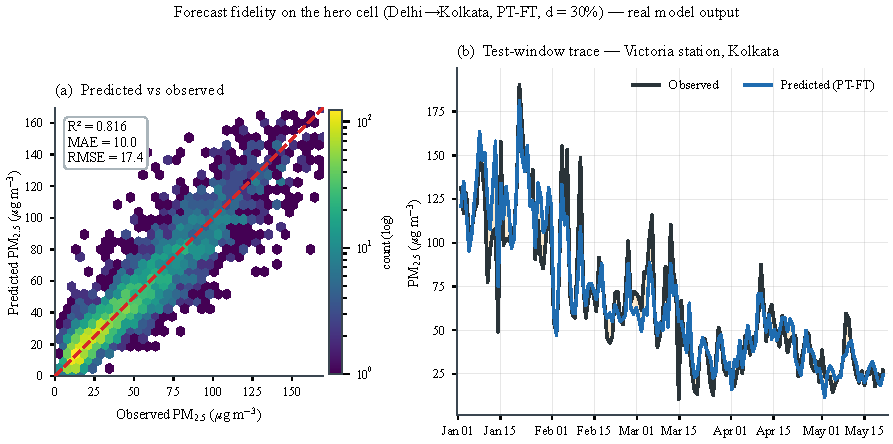
\includegraphics[width=\textwidth]{fig6_forecast.pdf}
\caption{Forecast fidelity on the hero transfer cell (Delhi$\rightarrow$Kolkata, PT-FT, $d=30\%$), real model output. (a) Predicted vs observed \pmf density with the 1:1 line. (b) Observed and predicted test-window trace for a representative Kolkata station, capturing the winter episode and its decay.}
\label{fig:forecast}
\end{figure*}

\subsection{Spatial Distribution of Skill}
A practical concern for any transferred forecaster is whether its skill is genuine network-wide or carried by a few well-behaved monitors. Fig.~\ref{fig:perstation} resolves the per-station error for the same hero cell: the transferred model attains $R^2=0.66$--$0.90$ and MAE $7$--$15$\ugm at \emph{every} one of the ten Kolkata stations, with the largest errors confined to the two highest-variance industrial sites (Padmapukur, Ghusuri) and uniformly strong skill elsewhere. The skill is therefore spatially distributed, not an artefact of a few easy stations --- a prerequisite for operational deployment across a city's whole network.

\begin{figure*}[!t]
\centering
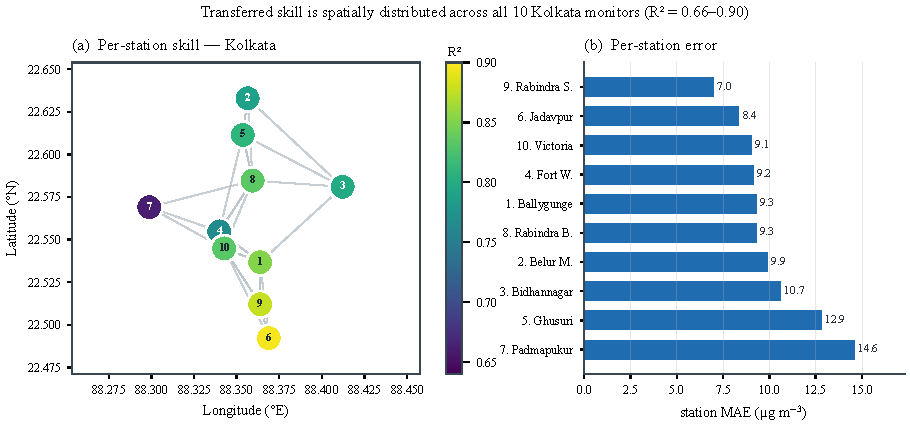
\includegraphics[width=\textwidth]{fig7_per_station.pdf}
\caption{Per-station skill of the transferred model on the target city (Delhi$\rightarrow$Kolkata, PT-FT, $d=30\%$). (a) The ten Kolkata monitors coloured by station-level $R^2$ (markers numbered, keyed to (b)); the $k$-NN graph edges are shown in grey. (b) Per-station MAE, sorted. Skill is distributed across the whole network, with the largest errors at the highest-variance industrial sites.}
\label{fig:perstation}
\end{figure*}

% =========================================================================
\section{Discussion}\label{sec:discussion}
% =========================================================================
\textbf{Accuracy is not the only axis.} PT-FT and Graph-DANN tie on forecast accuracy, but Graph-DANN additionally guarantees a city-invariant pooled embedding. This matters for tasks beyond single-pair accuracy: zero-target-label deployment (where a new city contributes only sensor features), cross-year robustness, and multi-source aggregation (the discriminator simply becomes a $k$-class problem). PT-FT cannot operate in the zero-label regime by construction.

\textbf{Why an inductive operator transfers across \V.} If two monitoring graphs are sampled from a similar generating process --- here, CPCB $k$-NN station graphs in the Indo-Gangetic Plain and its Brahmaputra extension --- an inductive GNN trained on one converges to nearly the same behaviour on the other as size grows \cite{ruiz2020graphon,levie2021transfer}. The 24/24 PT-FT pass rate validates this empirically in the tested regime.

\textbf{Operational implication.} A city with $\leq$10 CPCB stations need not train a dedicated deep forecaster: a Delhi-pretrained encoder fine-tuned on $d=30\%$ of the new city's data recovers \Rtwo within 0.04 of a fully-supervised model, at a fine-tune cost of minutes on commodity CPU. This is directly deployable as a standard operating procedure for under-monitored Tier-2/3 cities.

% =========================================================================
\section{Limitations}\label{sec:limitations}
% =========================================================================
Three cities is a small sample; generalization to other airsheds remains to be tested, and the graphon argument is suggestive, not conclusive. Kolkata and Guwahati have a single year of data, necessitating the interleaved split, which inflates absolute \Rtwo versus chronological-block cross-validation (method-vs-method rankings, which share the protocol, are unaffected); a chronological-block sensitivity analysis is the highest-priority follow-up. Per-cell metrics use a single seed; seed sweeps with Diebold--Mariano testing would tighten the Stage-1-vs-Stage-2 comparison. Finally, the encoder uses a single-head GAT; a GATv2 upgrade may further narrow the absolute-accuracy gap to LSTM-TL without changing the structural-transfer conclusion.

% =========================================================================
\section{Conclusion}\label{sec:conclusion}
% =========================================================================
We presented an inductive spatio-temporal GNN with two complementary cross-city transfer mechanisms for the practical regime of Indian \pmf forecasting, where source and target cities differ in monitoring-station count by an order of magnitude. We first established that transfer learning is a decisive lever for data-scarce cities using a station-independent LSTM, then showed that its station-independent form caps how far transfer can go, and finally closed that gap with an inductive encoder whose $\approx$25k parameters transfer verbatim from a 40-station to a 4-station graph. Across the full grid we obtain 24/24 (PT-FT) and 23/24 (Graph-DANN) verified knowledge-transfer passes; Graph-DANN further contributes a city-invariant embedding for zero-label and multi-source extensions. The work is accompanied by a complete leakage/overfitting audit and is reproducible on CPU-only hardware.

\section*{Acknowledgment}
The authors gratefully acknowledge the Central Pollution Control Board (CPCB), Government of India, for providing the open Continuous Ambient Air Quality Monitoring (CAAQM) data used in this study, and the Indian Institute of Information Technology Sri City for compute and supervision. The authors also acknowledge the use of a generative artificial-intelligence assistant for code scaffolding, figure generation, and language editing; all study design, experiments, analyses, and conclusions were conceived, executed, and verified by the authors, who take full responsibility for the content.

\section*{Author Contributions}
B.~Maitra led the implementation, software, experiments, data-leakage audit, and manuscript preparation. S.~Mondal contributed the methodology and formal analysis. M.~Thakur provided supervision, conceptualization, and critical review. All authors approved the final manuscript.

\section*{Funding}
This work received no external funding.

\section*{Conflict of Interest}
The authors declare no conflict of interest.

% =========================================================================
\begin{thebibliography}{00}
\bibitem{hei2024} Health Effects Institute, \emph{State of Global Air 2024}, Boston, MA, USA, 2024.
\bibitem{iqair2024} IQAir, \emph{2023 World Air Quality Report}, 2024.
\bibitem{who2021} World Health Organization, \emph{WHO Global Air Quality Guidelines}, Geneva, Switzerland, 2021.
\bibitem{wang2020pm25gnn} S. Wang, Y. Li, J. Zhang, Q. Meng, L. Meng, and F. Gao, ``PM2.5-GNN: A domain knowledge enhanced graph neural network for PM2.5 forecasting,'' in \emph{Proc. 28th Int. Conf. Adv. Geogr. Inf. Syst. (SIGSPATIAL)}, 2020, pp. 163--166.
\bibitem{chen2021gagnn} L. Chen \emph{et al.}, ``Group-aware graph neural network for nationwide city air quality forecasting,'' \emph{arXiv:2108.12238}, 2021.
\bibitem{shao2021highair} X. Shao, C. Zhang, T. Yan, and Z. Li, ``HighAir: A hierarchical graph neural network-based air quality forecasting method,'' \emph{arXiv:2101.04264}, 2021.
\bibitem{liang2023airformer} Y. Liang \emph{et al.}, ``AirFormer: Predicting nationwide air quality in China with transformers,'' in \emph{Proc. AAAI Conf. Artif. Intell.}, 2023, pp. 14329--14337.
\bibitem{wang2019regiontrans} L. Wang, X. Geng, X. Ma, F. Liu, and Q. Yang, ``Cross-city transfer learning for deep spatio-temporal prediction,'' in \emph{Proc. 28th Int. Joint Conf. Artif. Intell. (IJCAI)}, 2019, pp. 1893--1899.
\bibitem{yao2019metast} H. Yao, Y. Liu, Y. Wei, X. Tang, and Z. Li, ``Learning from multiple cities: A meta-learning approach for spatial-temporal prediction,'' in \emph{Proc. World Wide Web Conf. (WWW)}, 2019, pp. 2181--2191.
\bibitem{lu2022stgfsl} B. Lu \emph{et al.}, ``Spatio-temporal graph few-shot learning with cross-city knowledge transfer,'' in \emph{Proc. 28th ACM SIGKDD}, 2022, pp. 1162--1172.
\bibitem{jin2022crosstres} Y. Jin, K. Chen, and Q. Yang, ``Selective cross-city transfer learning for traffic prediction via source city region re-weighting,'' in \emph{Proc. 28th ACM SIGKDD}, 2022, pp. 731--741.
\bibitem{jin2023transgtr} Y. Jin, K. Chen, and Q. Yang, ``Transferable graph structure learning for graph-based traffic forecasting across cities,'' in \emph{Proc. 29th ACM SIGKDD}, 2023, pp. 1032--1043.
\bibitem{tang2022dastnet} Y. Tang \emph{et al.}, ``Domain adversarial spatial-temporal network: A transferable framework for short-term traffic forecasting across cities,'' in \emph{Proc. 31st ACM Int. Conf. Inf. Knowl. Manage. (CIKM)}, 2022, pp. 1905--1915.
\bibitem{hamilton2017graphsage} W. L. Hamilton, R. Ying, and J. Leskovec, ``Inductive representation learning on large graphs,'' in \emph{Adv. Neural Inf. Process. Syst. (NeurIPS)}, 2017, pp. 1024--1034.
\bibitem{velickovic2018gat} P. Veli\v{c}kovi\'c \emph{et al.}, ``Graph attention networks,'' in \emph{Proc. Int. Conf. Learn. Represent. (ICLR)}, 2018.
\bibitem{xu2019gin} K. Xu, W. Hu, J. Leskovec, and S. Jegelka, ``How powerful are graph neural networks?'' in \emph{Proc. Int. Conf. Learn. Represent. (ICLR)}, 2019.
\bibitem{ganin2016dann} Y. Ganin \emph{et al.}, ``Domain-adversarial training of neural networks,'' \emph{J. Mach. Learn. Res.}, vol. 17, no. 59, pp. 1--35, 2016.
\bibitem{tzeng2017adda} E. Tzeng, J. Hoffman, K. Saenko, and T. Darrell, ``Adversarial discriminative domain adaptation,'' in \emph{Proc. IEEE Conf. Comput. Vis. Pattern Recognit. (CVPR)}, 2017, pp. 7167--7176.
\bibitem{demathelin2020adversarial} A. de Mathelin, M. Atiq, G. Richard \emph{et al.}, ``Adversarial weighting for domain adaptation in regression,'' \emph{arXiv:2006.08251}, 2020.
\bibitem{yu2018stgcn} B. Yu, H. Yin, and Z. Zhu, ``Spatio-temporal graph convolutional networks: A deep learning framework for traffic forecasting,'' in \emph{Proc. 27th Int. Joint Conf. Artif. Intell. (IJCAI)}, 2018, pp. 3634--3640.
\bibitem{wu2019graphwavenet} Z. Wu, S. Pan, G. Long, J. Jiang, and C. Zhang, ``Graph WaveNet for deep spatial-temporal graph modeling,'' in \emph{Proc. 28th Int. Joint Conf. Artif. Intell. (IJCAI)}, 2019, pp. 1907--1913.
\bibitem{bai2018tcn} S. Bai, J. Z. Kolter, and V. Koltun, ``An empirical evaluation of generic convolutional and recurrent networks for sequence modeling,'' \emph{arXiv:1803.01271}, 2018.
\bibitem{ruiz2020graphon} L. Ruiz, L. F. O. Chamon, and A. Ribeiro, ``Graphon neural networks and the transferability of graph neural networks,'' in \emph{Adv. Neural Inf. Process. Syst. (NeurIPS)}, 2020, pp. 1702--1712.
\bibitem{levie2021transfer} R. Levie, W. Huang, L. Bucci, M. Bronstein, and G. Kutyniok, ``Transferability of spectral graph convolutional neural networks,'' \emph{J. Mach. Learn. Res.}, vol. 22, no. 272, pp. 1--59, 2021.
\bibitem{yosinski2014} J. Yosinski, J. Clune, Y. Bengio, and H. Lipson, ``How transferable are features in deep neural networks?'' in \emph{Adv. Neural Inf. Process. Syst. (NeurIPS)}, 2014, pp. 3320--3328.
\bibitem{yadav2024} P. Yadav, A. Kumar, V. Sharma, and A. Verma, ``Cross-year deep transfer learning with attention for Delhi PM2.5 forecasting,'' \emph{Environ. Model. Softw.}, vol. 175, p. 105987, 2024.
\bibitem{sangiorgio2024} M. Sangiorgio and G. Guariso, ``Transfer learning in environmental data-driven models: Ozone forecast in the Alpine region,'' \emph{Environ. Model. Softw.}, vol. 177, p. 106048, 2024.
\bibitem{bergmeir2018cv} C. Bergmeir, R. J. Hyndman, and B. Koo, ``A note on the validity of cross-validation for evaluating autoregressive time series prediction,'' \emph{Comput. Stat. Data Anal.}, vol. 120, pp. 70--83, 2018.
\bibitem{btp2025} B. Maitra, ``Transfer learning framework for PM2.5 forecasting in Indian cities,'' B.Tech. thesis, Indian Inst. Inf. Technol. Sri City, India, 2025.
\bibitem{long2012dtl} M. Long, J. Wang, G. Ding, W. Cheng, X. Zhang, and W. Wang, ``Dual transfer learning,'' in \emph{Proc. SIAM Int. Conf. Data Mining (SDM)}, 2012, pp. 540--551.
\bibitem{long2018cdan} M. Long, Z. Cao, J. Wang, and M. I. Jordan, ``Conditional adversarial domain adaptation,'' in \emph{Adv. Neural Inf. Process. Syst. (NeurIPS)}, 2018, pp. 1640--1650.
\bibitem{chen2021rsd} X. Chen, S. Wang, J. Wang, and M. Long, ``Representation subspace distance for domain adaptation regression,'' in \emph{Proc. Int. Conf. Mach. Learn. (ICML)}, 2021, pp. 1749--1759.
\bibitem{long2017jan} M. Long, H. Zhu, J. Wang, and M. I. Jordan, ``Deep transfer learning with joint adaptation networks,'' in \emph{Proc. Int. Conf. Mach. Learn. (ICML)}, 2017, pp. 2208--2217.
\bibitem{zhu2021dsan} Y. Zhu \emph{et al.}, ``Deep subdomain adaptation network for image classification,'' \emph{IEEE Trans. Neural Netw. Learn. Syst.}, vol. 32, no. 4, pp. 1713--1722, 2021.
\end{thebibliography}

\end{document}
